\documentclass[10pt,aspectratio=169]{beamer}

\usepackage{spbu}

\usepackage[T2A]{fontenc}
\usepackage[utf8]{inputenc}
\usepackage[english,russian]{babel}
\usepackage{ulem}

\title{\LaTeX}
\subtitle{Введение}


\begin{document}

    \maketitle

    \section{Введение}
    
    \begin{frame}{\TeX}
    	\begin{columns}
    		\begin{column}{0.6\textwidth}
    			\begin{itemize}
    			\item TeX или \TeX \hspace{0.4mm} --- система компьютерной верстки, разработанная американским профессором информатики Дональдом Кнутом в целях создания компьютерной типографии. В неё входят средства для секционирования документов, для работы с перекрёстными ссылками. В частности, благодаря этим возможностям, TeX популярен в академических кругах, особенно среди математиков и физиков.
    			\item Первый выпуск --- 1978 год.
    			\end{itemize}
    		\end{column}
    		\begin{column}{0.25\textwidth}
    			\begin{figure}[h!]
    				\centering
    				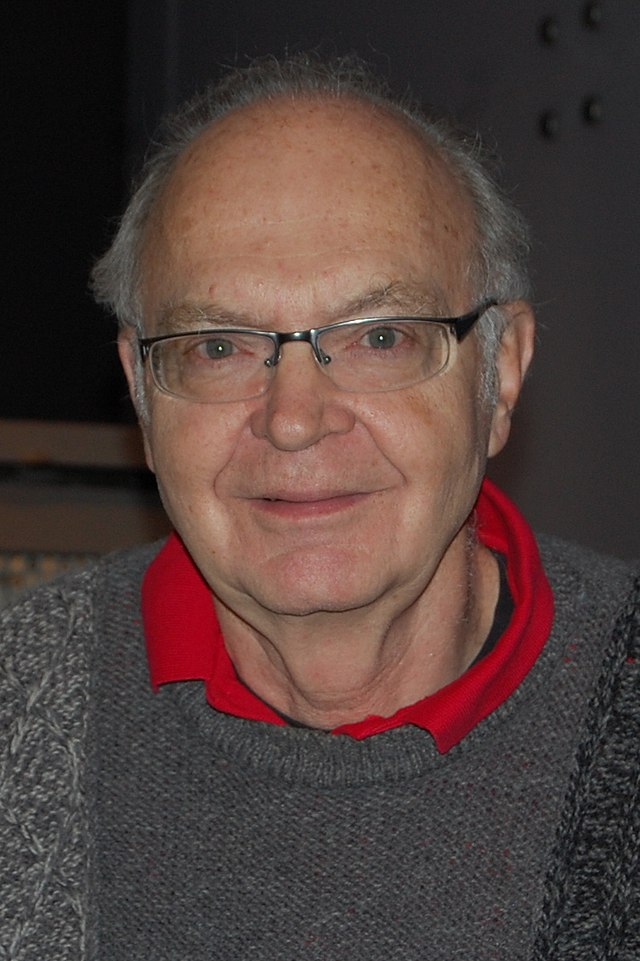
\includegraphics[width=\textwidth]{img/knuth.jpg}
    				\caption{Дональд Кнут}
    				\label{fig:knuth}
    			\end{figure}
    		\end{column}
    	\end{columns}
    \end{frame}
    
    \begin{frame}{LaTeX}
   		\begin{columns}
    		\begin{column}{0.63\textwidth}
		    	\begin{itemize}
		          	\item LaTeX --- наиболее популярный набор макрорасширений системы компьютерной верстки \TeX, который облегчает набор сложных документов. В типографском наборе системы \TeX \hspace{0.4mm} форматируется традиционно как \LaTeX.
		          	\item Первый выпуск --- 1984 год.
		          	\item Текущая глобальная версия 2$\varepsilon$.
		          	\item Официальный сайт: \url{https://latex-project.org}.
		    	\end{itemize}
    		\end{column}
    		\begin{column}{0.25\textwidth}
    			\begin{figure}[h!]
   				\centering
   				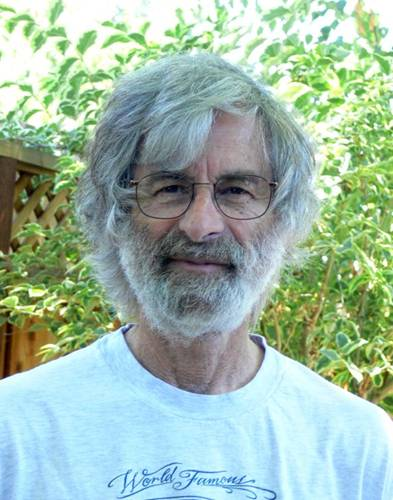
\includegraphics[width=\textwidth]{img/lamport.jpg}
   				\caption{Лесли Лэмпорт}
   				\label{fig:lamport}
   			\end{figure}
   			\end{column}
   		\end{columns}
    \end{frame}
    
    \begin{frame}{Произношение}
    	\begin{figure}[h!]
    		\centering
    		
\includegraphics[scale=0.25]{img/megabrain.png}
    		\label{fig:megabrain}
		\end{figure}
   	\end{frame}
    
    \begin{frame}{MS Word или \LaTeX}
    	\begin{columns}
	    	\begin{column}{0.5\textwidth}
	    		\begin{itemize}
	    			\item WYSIWYG vs Язык разметки
	    			\item Совместимость
	    			\item Библиография, перекрестные ссылки
	    			\item Рисунки
	    			\item Формулы
	    		\end{itemize}
	    	\end{column}
	    	\begin{column}{0.5\textwidth}
	    		\begin{figure}[h!]
	    			\centering
	    			
\includegraphics[scale=0.08]{img/word-latex.png}
	    		\end{figure}
	    	\end{column}
    	\end{columns}
    \end{frame}
    
    \begin{frame}{Литература}
    	\begin{itemize}
    		\item Кнут Д. Все про \TeX
    		\item Львовский С. М. Набор и верстка в системе \LaTeX
    		\item TikZ Manual for Version 2.0
    		\begin{itemize}
    			\item The TikZ and PGF Packages Manual for Version 3.1.10 \url{https://tikz.dev}
    		\end{itemize}
    		\item Воронцов К. В. \LaTeX $2{\varepsilon}$ в примерах
    	\end{itemize}
    \end{frame}
    
    \begin{frame}{Дистрибутивы}
    	\begin{itemize}
    		\item MikTeX \url{https://miktex.org}
    		\item TeX Live \url{https://tug.org/texlive}
    		\item MacTeX \url{https://tug.org/mactex}
    	\end{itemize}
    \end{frame}
    
    \begin{frame}{Редакторы/среды}
    	Ориентированные на LaTeX
    	\begin{itemize}
    		\item Overleaf, Online LaTeX Editor: \url{https://www.overleaf.com}
    		\item TeXstudio: \url{https://www.texstudio.org}
    		\item WinEdt, WinEdt 11: \url{https://www.winedt.com}
    		\begin{itemize}
    			\item \url{https://rutracker.org/forum/viewtopic.php?t=3865802}
    		\end{itemize}
    		\item Texmaker: \url{https://www.xm1math.net/texmaker}
    		\item TeXworks: \url{https://www.tug.org/texworks}
    	\end{itemize}
    	Общего назначения
    	\begin{columns}
    		\begin{column}{0.5\textwidth}
		    	\begin{itemize}
		    		\item{Vim}
		    		\item{Visual Studio Code}
		    	\end{itemize}
	    	\end{column}
	    	\begin{column}{0.5\textwidth}
		    	\begin{itemize}
		    		\item{Sublime Text}
	    			\item{Atom}
		    	\end{itemize}
	    	\end{column}
    	\end{columns}
    \end{frame}

    \section{Общие положения}

    \begin{frame}[fragile]{Структура документа}
        Для создания простейшего документа с использованием \LaTeX \vspace{0.4mm} достаточно воспользоваться следующим кодом.
        \begin{block}{Минимальный документ}
\begin{lstlisting}
\documentclass{article}			% Преамбула
\begin{document}					
	Hello, world!				% Документ
\end{document}
\end{lstlisting}
        \end{block}
        
        
    \end{frame}
    
    \begin{frame}[fragile]{Синтаксис}
    	Основной синтаксис
    	\begin{itemize}
    		\item Команды: \verb|\command[optional]{arguments}|
    		\item Окружения:
\begin{lstlisting}
\begin{environment}					
	Содержимое окружения...
\end{environment}
\end{lstlisting}
			\item Группировка: \verb|Содержимое 1 {Содержимое 2}|
    	\end{itemize}
    	Специальные символы
    	\begin{itemize}
    		\item \verb|# $ % & _ { } ~ ^ \|
    		\item экранирование \verb|\# \$ \% \& \_ \{ \}|
    	\end{itemize}
    \end{frame}
    
   	\section{Преамбула}
    
    \begin{frame}[fragile]{Содержимое преамбулы}
   		\begin{block}{Пример 1}
\begin{lstlisting}
\documentclass[12pt]{article} 		% Документ принадлежит классу article,
									% а также будет печататься в 12 пунктов

\usepackage[russian]{babel} 		% Пакет поддержки русского языка

\title{Полиномы Чебышева} 			% Заглавие документа
\date{\today} 						% Дата создания
\end{lstlisting}
		\end{block}
		На основании значений аргументов команд \verb|\title| и \verb|\date| можно построить титульный лист/шапку с использованием команды \verb|\maketitle|.
   		\begin{block}{Пример 2}
\begin{lstlisting}
\documentclass[11pt,a4paper,oneside]{report} 		
\usepackage{pslatex,palatino,avant,graphicx,color}
\usepackage[margin=2cm]{geometry}
\end{lstlisting}
		\end{block}
   	\end{frame}
   	
    \begin{frame}[fragile]{Document Class}
    	\begin{itemize}
    	\item Стандартные классы:
	   		\begin{itemize}
	   			\item article,
	   			\item report,
	   			\item book,
	   			\item letter,
	   			\item disser.
	   		\end{itemize}
   		
   		\item Как правило, разные классы предоставляют одинаковые или похожие “команды”, но результат получается разный.
   		
   		\item Есть возможность написания своих классов.
   		\end{itemize}
   	\end{frame}
   	
   	\begin{frame}[fragile]{Каркас страницы}
   		\begin{columns}
   			\begin{column}{0.5\textwidth}
   				\begin{itemize}
   					\item Для ручного управления этими параметрами используется пакет \verb|geometry|.
   					\item В преамбуле \verb|\usepackage[margin=3cm]{geometry}|.
   					\item Варианты:
   					\begin{itemize}
   						\item top,
   						\item bottom,
   						\item left,
   						\item right.
   					\end{itemize}
   					\item Подробнее можно посмотреть
   					\href{https://texdoc.org/serve/geometry.pdf/0}{тут}.
   				\end{itemize}
   			\end{column}
   			\begin{column}{0.3\textwidth}
   				\begin{figure}
   					\centering
   					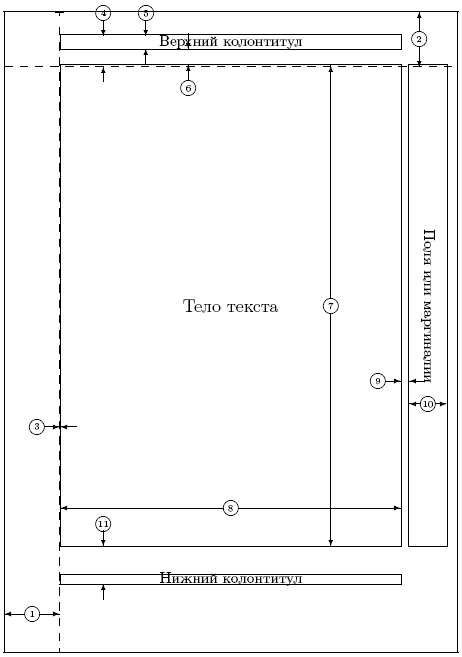
\includegraphics[scale=0.25]{img/skeleton.png}
   					\caption{Каркас страницы}
   					\label{fig:skeleton}
   				\end{figure}
   			\end{column}
   		\end{columns}
   	\end{frame}
   	
   	\section{Содержание документа}
   	
    \begin{frame}[fragile]{Переносы, деление на абзацы}
   		\begin{itemize}
   			\item Двойной конец строки (пустая строка) --- конец абзаца.
   			\item Две и более пустые строки --- все равно, что одна.
   			\item Лишние пробелы и пробелы в начале строк игнорируются.
   			\item \verb|\\| --- перенос на новую строку.
   			\begin{itemize}
   				\item Можно передать величину вертикального отступа в
   				качестве опционального аргумента: \verb|\\[1cm]|.
   			\end{itemize}
   			\item Команда \verb|\linebreak| --- разрыв строки.
   			\item Команда \verb|\pagebreak| --- разрыв страницы.
   			\item Если необходимо начать абзац без красной строки: \verb|\noindent|.
   		\end{itemize}
   	\end{frame}
   	
    \begin{frame}[fragile]{Пробелы, межстрочные интервалы}
   		\begin{itemize}
   			\item \verb|\|, \verb|\,|, \verb|\!|, \verb|\quad|,
   			\item \verb|\hfill|,
   			\item \verb|\vspace{}|, \verb|\hspace{}|.
   		\end{itemize}
   	\end{frame}
   	
   	
    \begin{frame}[fragile]{Списки}
    	Три основные окружения для создания списков: \verb|itemize|, \verb|enumerate|, \verb|description|.
   		\begin{itemize}
   			\item \verb|\item| начинает новый элемент списка.
   			\item \verb|\item| должен быть первой командой окружения.
   			\item Списки могут быть вложенными.
   			\item В \verb|description| элемента по умолчанию не нумеруются/не маркеруются.
   			\item Можно изменить маркер \verb|\item[example A]|.
   		\end{itemize}
   	\end{frame}
   	
    \begin{frame}[fragile]{Списки}
    	\framesubtitle{Примеры}
		\begin{columns}
   			\begin{column}{0.5\textwidth}
\begin{lstlisting}
\begin{itemize}
	\item[$\dagger$] пункт 1
	\item пункт 2
	\begin{itemize}
		\item подпункт 2.1
		\item подпункт 2.2
	\end{itemize}
	\item пункт 3
\end{itemize}
\end{lstlisting}
   			\end{column}
   			\begin{column}{0.3\textwidth}
   				\begin{itemize}
   					\item[$\dagger$] пункт 1
   					\item пункт 2
   					\begin{itemize}
   						\item подпункт 2.1
   						\item подпункт 2.2
   					\end{itemize}
   					\item пункт 3
   				\end{itemize}
   			\end{column}
   		\end{columns}
   		\begin{columns}
   			\begin{column}{0.5\textwidth}
\begin{lstlisting}
\begin{description}
	\item[описание 1] пункт 1
	\item[пример] пункт 2
	\item пункт 3
	\item пункт 4
\end{description}
\end{lstlisting}
			\end{column}
   			\begin{column}{0.3\textwidth}
   				\begin{description}
   					\item[описание 1] пункт 1
   					\item[пример] пункт 2
   					\item пункт 3
   				\end{description}
   			\end{column}
   		\end{columns}
   	\end{frame}
   	
    \begin{frame}[fragile]{Иерархия содержания документа}
    	\framesubtitle{На примере класса disser}
   		Для организации иерархии в классе \verb|disser| используются команды: 
   		\begin{itemize}
   			\item \verb|chapter|,
   			\item \verb|section|,
   			\item \verb|subsection|,
   			\item \verb|subsubsection|.
   		\end{itemize}
   	\end{frame}

    \begin{frame}[fragile]{Форматирование текста}
		\framesubtitle{Шрифты}
		Для представления различной информации, уместно использовать соответствующее форматирование шрифта:
		\begin{itemize}
			\item {\verb|\textrm{}|: \textrm{стандартный шрифт;}}
			\item {\verb|\textsf{}|: \textsf{шрифт семейства sans-serif;}}
			\item {\verb|\texttt{}|: \texttt{моноширинный шрифт.}}
			\item {\verb|\textbf{}|: \textbf{полужирный шрифт.}}
			\item {\verb|\textit{}|: \textit{курсив.}}
			\item {\verb|\textrm{}|: \textrm{\sout{Times New} Roman.}}
			\item и др.
		\end{itemize}
	\end{frame}
	
 	\begin{frame}[fragile]{Форматирование текста}
		\framesubtitle{Выравнивание текста}
		Для выравнивания текста следует использовать окружения:
		\begin{itemize}
			\item \verb|center|,
			\item \verb|flushleft|,
			\item \verb|flushright|.
		\end{itemize}
	\end{frame}

 	\begin{frame}[fragile]{Форматирование текста}
		\framesubtitle{Размер шрифта}
		\begin{itemize}
			\item По умолчанию используется шрифт в 10 пунктов.
			\item Можно поменять, задав аргумент классу документа: \verb|\documentclass[12pt,a4paper]{article}|
			\item Класс \verb|article| поддерживает шрифт в 9, 10, 11, 12
			пунктов.
			\item Можно изменять шрифт с помощью команд: \verb|tiny|, \verb|scriptsize|, \verb|footnotesize|, \verb|small|, \verb|normalsize|, \verb|large|, \verb|Large|, \verb|LARGE|, \verb|huge|, \verb|Huge|.
		\end{itemize}
		
		{\tiny tiny }
		{\scriptsize scriptsize }
		{\footnotesize footnotesize }
		{\small small}
		{\normalsize normalsize}
		{\large large }
		{\Large Large}
		{\LARGE LARGE}
		{\huge huge}
		{\Huge Huge}
	\end{frame}
	
 	\begin{frame}[fragile]{Русский язык}
		\framesubtitle{Пунктуация}
		\begin{itemize}
			\item \verb|-|, \verb|--|, \verb|---|, \verb|$-$|.
			\item Кавычки --- «елочки»: \verb|<<| и \verb|>>|.
			\item В большинстве случаев \LaTeX правильно расставляет переносы. В сложных случаях стоит помочь при помощи команды \verb|\-|.
		\end{itemize}
		
		\begin{itemize}
			\item Лебедев А. Ководство
			\begin{itemize}
				\item \url{https://www.artlebedev.ru/kovodstvo/sections/97}
			\end{itemize}
			\item Мильчин А., Людмила Ч. Справочник издателя и автора
			\begin{itemize}
				\item \url{https://www.artlebedev.ru/izdal/spravochnik-izdatelya-i-avtora}
			\end{itemize}
		\end{itemize}
	\end{frame}
	
	\section{Заключение}
	
 	\begin{frame}[fragile]{Источники}
		\begin{itemize}
			\item Репозиторий на GitHub:
				\url{https://github.com/gleb-kun/mpt-course/tree/master/latex}
    		\item Кнут Д. Все про \TeX
			\item Львовский С. М. Набор и верстка в системе \LaTeX
			\item TikZ Manual for Version 2.0
			\begin{itemize}
				\item The TikZ and PGF Packages Manual for Version 3.1.10 \url{https://tikz.dev}
			\end{itemize}
			\item Воронцов К. В. \LaTeX $2{\varepsilon}$ в примерах
			\item Коробейников А. И. Презентации \url{https://statmod.ru/wiki/study:fall2018:tex}
			\item Лебедев А. Ководство
			\begin{itemize}
			\item \url{https://www.artlebedev.ru/kovodstvo/sections/97}
			\end{itemize}
			\item Мильчин А., Людмила Ч. Справочник издателя и автора
			\begin{itemize}
				\item \url{https://www.artlebedev.ru/izdal/spravochnik-izdatelya-i-avtora}
			\end{itemize}
		\end{itemize}
	\end{frame}

    \backmatter

\end{document}
